\documentclass[border={0 25mm 0 0}]{standalone}
\usepackage{tikz}
\usetikzlibrary{calc, positioning}

\begin{document}
	
	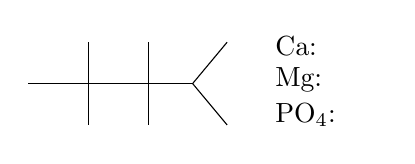
\begin{tikzpicture}[node distance=0.5mm]
		\def\blank{Y};
		\ifx\blank\empty
			\tikzstyle{data} = [black]
			\def\na{Na};
			\def\k{K};
			\def\cl{Cl};
			\def\bicarb{HCO3};
			\def\bun{BUN};
			\def\cr{Cr};
			\def\glu{Glu};
			\def\drawcamgphos{Y};
			\def\ca{Ca};
			\def\mg{Mg};
			\def\phos{P};
		\else
			\tikzstyle{data} = [white]
			\def\na{152};
			\def\k{3.7};
			\def\cl{108};
			\def\bicarb{28};
			\def\bun{25};
			\def\cr{0.8};
			\def\glu{327};
			\def\drawcamgphos{Y};
			\def\ca{10.8};
			\def\mg{2.8};
			\def\phos{4.0};
		\fi

		\coordinate (center1) at (0,0);
		\node[data, above of=center1, anchor=south] (na) {\na};
		\node[data, below of=center1, anchor=north] (k) {\k};

		\coordinate[right of=center1, xshift=7mm] (center2);
		\node[data, above of=center2, anchor=south] (cl) {\cl};
		\node[data, below of=center2, anchor=north] (hco3) {\bicarb};

		\coordinate[right of=center2, xshift=7mm] (center3);
		\node[data, above of=center3, anchor=south] (bun) {\bun};
		\node[data, below of=center3, anchor=north] (cr) {\cr};

		\node[data, right of=center3, xshift=2mm, anchor=west] (glu) {\glu};
		\coordinate[right of=center3, xshift=1.5mm] (center4);

		\draw
			let 
				\p1 = (na.north east),
				\p2 = (k.south east),
				\p3 = (cl.north west),
				\p4 = (hco3.south west)
			in
				({(max(\x1,\x2)+min(\x3,\x4))/2},\y1) -- ({(max(\x1,\x2)+min(\x3,\x4))/2},\y2);
		\draw
			let 
				\p1 = (cl.north east),
				\p2 = (hco3.south east),
				\p3 = (bun.north west),
				\p4 = (cr.south west)
			in
				({(max(\x1,\x2)+min(\x3,\x4))/2},\y1) -- ({(max(\x1,\x2)+min(\x3,\x4))/2},\y2);
		\draw
			let 
				\p1 = (bun.north east),
				\p2 = (glu),
				\p3 = (center4)
			in
				(\x3,\y2) -- (\x2,\y1);
		\draw
			let 
				\p1 = (cr.south east),
				\p2 = (glu),
				\p3 = (center4)
			in
				(\x3,\y2) -- (\x2,\y1);
		\draw
			let
				\p1 = (na.north west),
				\p2 = (k.south west),
				\p3 = (center4)
			in
				({min(\x1,\x2)},\y3) -- (center4);

		\coordinate (center5) at ($(glu.east)+(0.1,0)$);
		\ifx\drawcamgphos\empty
			%
		\else
			\node[above of=center5, anchor=west] (mg) {Mg:};
			\node[data, right=of mg, anchor=west, xshift=-6] {\mg};
			\node[anchor=south west] (ca) at ($(mg.north west)+(0,-0.1)$) {Ca:};
			\node[data, right=of ca, anchor=west, xshift=-6] {\ca};
			\node[anchor=north west] (phos) at ($(mg.south west)+(0,0.1)$) {PO$_4$:};
			\node[data, right=of phos, anchor=west, xshift=-6] {\phos};
		\fi
	\end{tikzpicture}

\end{document}